%%%%%%%%%%%%%%%%%%%%%%%%%%%%%%%%%%%%%%%%%%%%%%%%%%%%%%%%%%%%%%%%%%%%%%%%%%%%%%%%%%%%%%%%%%%%%
% 																	INTRODUCTION																						%
%%%%%%%%%%%%%%%%%%%%%%%%%%%%%%%%%%%%%%%%%%%%%%%%%%%%%%%%%%%%%%%%%%%%%%%%%%%%%%%%%%%%%%%%%%%%%

%%%%%%%%%%%%%%%%%%%%%%%%%%%%%%%%%%%%%%%%%%%%%%%%%%%%%%%%%%%%%%%%%%%%%%%%%%%%%%%%%%%%%%%%%%%%%
% 															Chapter Introduction  																			%
%%%%%%%%%%%%%%%%%%%%%%%%%%%%%%%%%%%%%%%%%%%%%%%%%%%%%%%%%%%%%%%%%%%%%%%%%%%%%%%%%%%%%%%%%%%%%
\chapter{INTRODUCTION}

The industrial manipulators are highly non-linear dynamic systems in general, so it becomes difficult to achieve the high-performance trajectory tracking. Though many methods have been proposed by different authors, the computed-torque control is the the most common control scheme that is suitable for this kind of a problem. In spite of having many process control methods for the industrial robots, the PID controller is selected as the process control method and it is briefly explained in the next section. The computed-torque control method is advantageous than the pure PID control in many aspects such as the trajectory tracking control performance, lower feedback gains, lower energy consumption and the compliant motion~\cite{4586493}. This work aims to achieve the advanced model based controller scheme where the linear feedback control system is mandatory. There are two important aspects considered in the computed-torque control are the control law and dynamic model. Though this method is effective in accurate trajectory tracking, the manipulator is subject to uncertainties even in a well-defined industrial setup such as the accuracy of the model parameters and the unmodeled dynamics~\cite{trajectorytracking_nn}. The first uncertainty in the manipulator is that the model parameters provided by the manufacturers, these parameters are not accurate-enough and the findings on the same are presented by many researchers~\cite{muggler2013torque}~\cite{Atkeson}. The second uncertainty in the manipulator is unmodeled dynamics i.e. friction. The accurate model of the robot is mandatory as discussed in the previous section and the unavailability of the joint-torque sensors~\cite{torquecontrol} in the youBot manipulator joints makes the tracking control problem even harder. Apparently, there are only limited advantages of the computed-torque control strategy where the accuracy of the model parameters are not good enough. So, the accurate model parameters of the links are mandatory to solve this problem and it has been widely investigated by many researchers~\cite{Atkeson}~\cite{swevers} where the authors propose the identification procedure that can be used to estimate the model parameters of the system but there are many challenges involved in achieving it due to the presence of the implicit conventions, semantic problems and the trajectory selection criteria. The modified recursive Newton-Euler formulation is used for this purpose and then model fitting methods can be used to identify the model parameters of the links. This work attempts to deploy the estimated model parameters along with the friction compensation that brings us close in obtaining the complete dynamics of the system which in-turn provides the robust trajectory tracking in high-speed operations. The control can be considered in two different spaces such as

\begin{itemize}
\item \textbf{Joint space control }The joint controller contains the feedback control system that makes sure that the execution of the expected motion is being closely followed by the joint coordinates.
\item Whereas \textbf{in task/operational space control}, it is important to achieve the precise control of the end-effector motion for which the compliant motion control is necessary. The compliant control is nothing but having a proper algorithm that relates the interaction of the end-effector and the environment appropriately.
\end{itemize}

This work uses the joint space controller, so the torques can be commanded to the manipulator joints for executing the desired motion and it does not regulate the forces. The commanded torques go through an additional safety control layer that is implemented around the computed-torque control scheme. This layer performs the checking in all the three modes such as position, velocity and torque which depends particularly on the encoder data before applying the commanded torques to the manipulator joints. Feed-forward torques are generated through ID solver which is readily available in orocos KDL~\cite{smits2011kdl} library and the kinematic chain of the youBot manipulator needs to be created manually. There are two possible independent-joint control designs that can be used in a controller such as the independent single-joint and multi-joint model~\cite{Chung2016}. The independent single-joint model considers the dynamics of a single joint and it's response. Whereas the multi-joint model based control design considers the complete dynamic model of the robot. This work uses the multi-joint model where the interaction among the joints are handled. The desired end-effector motion can be executed by commanding the appropriate torques to the manipulator joints which depends on the motion plan in the joint level.

\section*{Mode of control}

The joint can be commanded with three kinds of inputs such as position, velocity and torque. So, a joint can be controlled in three different modes as depicted in Fig.~\ref{fig:modeofcontrol}.

\begin{figure}[h]
\centering
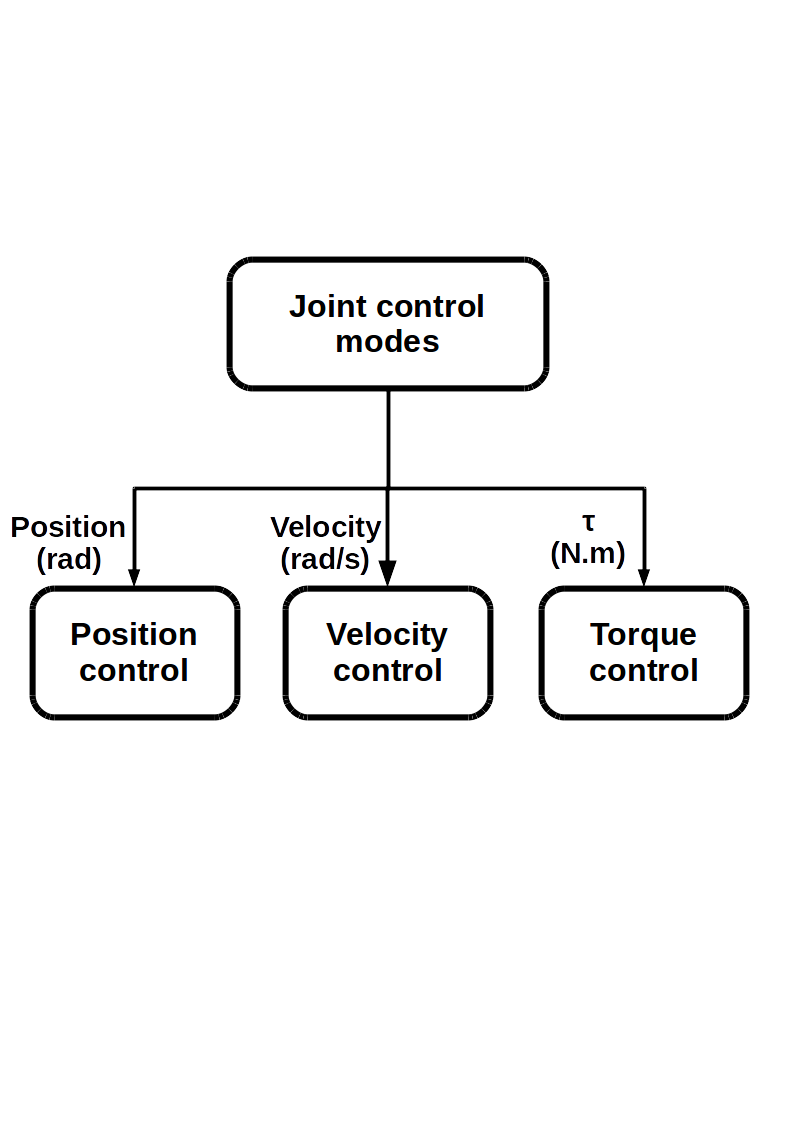
\includegraphics[width=80mm, trim=0 300 0 200]{pictures/joint_control_mode}
\caption{Joint's mode of control}
\label{fig:modeofcontrol}
\end{figure}

In position mode, a joint is commanded with position (joint angle in radians) to move the joint from a particular position to an another position. Whereas, the velocity mode commands the velocity to the joints for achieving the desired motion. The final classification is the torque control mode that commands the torque to the manipulator joints. The trajectory tracking errors can be efficiently minimized via torque mode since the dynamics and the joint configuration is considered~\cite{muggler2013torque}. Since, the motor takes the current as an input, the commanded joint torque has to be converted to target currents using a motor model based on the following equation~\eqref{eq:torquetocurrent}.

\begin{equation}
Current = (Commanded\_torque \times Gear\_ratio) / Torque\_constant (ampere)
\label{eq:torquetocurrent}
\end{equation}

The inverse of the above equation converts the current that is measured from the motors into joint torque. 

\begin{equation}
Torque= (Current \times Torque\_constant) / Gear\_ratio (Newton meters)
\label{eq:currenttotorque}
\end{equation}

The current to torque conversion as specified in the equation~\eqref{eq:currenttotorque} is particularly useful in interpreting the results of the system easily. The equations~\eqref{eq:torquetocurrent}~\eqref{eq:currenttotorque} are given based on the youbot driver\protect\footnotemark that is used in this work. \footnotetext[1]{\url{https://github.com/youbot/youbot_driver}} The torque control is quite robust and follows the trajectories in an accurate manner. This work uses the advanced model based torque controller and it is implemented in the joint space rather than the task space. This helps us in executing/tracking the trajectories in an accurately. This work assumes that the existing joint level controller gains are optimum hence the tuning the controller gains in the joint level is not the primary focus.

\section*{Control systems overview}
Basic definitions of this section are referred from~\cite{sellers2001overview}~\cite{astrom1995pid}. A system is considered to be linear when a change in output is directly proportional to the change in input. Since the robotic systems are highly non-linear, it is important to have the linear control strategy. This is achieved by using the linearization techniques that solves the non-linear systems problem. There are two kinds of control systems available such as open loop and the closed loop systems. Open loop, closed loop systems are depicted in the figures 1.2, 1.3 respectively. In the open loop systems, inputs are given to the system and the outcome is accepted regardless the deviations in the desired behaviour (feedback is not considered).

\begin{center}
\vspace{0.5cm}
\begin{tikzpicture}[auto, node distance=2cm,>=latex']
    \node [input, name=input] {};
    \node [block, right of=input, node distance=2.5cm] (robot){\textbf{Robot}};
	\node [output, right of=robot, node distance=2.9cm](output){};
	\draw [->,thick] (input) -- node {Desired} (robot);
    \draw [->,thick] (robot) -- node[pos=0.5] {Measured} (output);
\end{tikzpicture}
\captionof{figure}{Open loop system}
\vspace{0.5cm}
\begin{tikzpicture}[auto, node distance=2cm,>=latex']
    \node [input, name=input] {};
    \node [sum, right of=input, node distance=1.5cm] (minus) {\textbf{-}};
    \node [block, right of=minus, node distance=2.5cm] (control){\textbf{Controller}};
    \node [block, right of=control,
            node distance=3.5cm] (robot) {\textbf{Robot}};
	\node [output, right of=robot, node distance=2.9cm](output){};
	\draw [->,thick] (input) -- node {SP} (minus);
	\draw [->,thick] (minus) -- node {error} (control);
    \draw [->,thick] (control) -- node {CV} (robot);
    \draw [->,thick] (robot) -- node[pos=0.5] {PV} (output);
	\draw [->,thick] (output) -- ++ (0,-1.3) -| node [] {} (minus);
\end{tikzpicture}
\captionof{figure}{Closed loop system}
\end{center}

Whereas, the closed-loop control systems account the feedback of the system to minimize the deviations between the desired and observed data. This work uses the closed loop system for achieving the precise control of the manipulators.

\subsection*{PID controller}
The PID controller is the most commonly used controller in many of the industrial applications due to it's simplicity and it offers a lot of advantages such as fast response, brings the steady state error close to zero, avoiding oscillations and to achieve the stability in the system~\cite{temelp}~\cite{Chung2016}. It is possible to change the steady state response of the closed-loop system using this controller. The PID controller computes the error value between the desired and measured set-points repeatedly and it applies the correction based on the proportional(P), integral(I) and derivative(D) terms. P-term represents the current error that is being observed. I-term represents the history of errors which will be used to minimize the error between the expected set-point and it's response. D term is considered to predict the error based on it's rate of change in error. D term counteracts the overshoot caused by the P and I terms. The general mathematical representation of the complete PID control function can be expressed as follows

\begin{equation}
PV(t) = K_p\cdot error(t) + K_i\cdot \int_{0}^{t} e(t') dt' + K_d\cdot \frac{de(t)}{dt}
\end{equation}

It is possible to use different combinations within this controller depending on the requirements such as

\begin{itemize}
\item \textbf{P only control} is used in some specific applications where the feedback is expected to be constant.
\item \textbf{PI control} is commonly used controller.
\item \textbf{PD control} is used to control the servo motors.
\end{itemize}

The terms that are commonly used in the controller is depicted in the figure 1.3 and it is explained below

\begin{itemize}
\item Process Variable(\textbf{PV}) is the actual feedback that is being fed back to the controller from a process/system. 
\item Set Point(\textbf{SP}) is the desired variable for the process variable that is discussed above.
\item Control Variable(\textbf{CV}) is the actual output of the controller where the P, I and D terms are getting computed.
\item Error(\textbf{e}) is computed by finding the difference between SP and PV which can be a position or velocity set-point.
\item $K_p, K_i, K_d$ represents the proportional, integral and the derivative gains of the controller.
\begin{itemize}
\item If $K_p$ is high, the system oscillates a lot before reaching the desired setpoint which inturn introduces an offset in the system. 
\item $K_i$ tend to counteract this offset introduced by P control. If this gain value is high, the setpoint reaches the process variable faster.
\item $K_d$ tends to keep the stability of the system in control.
\end{itemize}
\end{itemize}

\subsubsection*{P control}

Proportional(P) control~\cite{temelp} is the linear feedback control system which produces an output that is proportion to the present error value(i.e. position set-point versus the control output). The proportion of the controller can be adjusted by multiplying the error with the proportional gain. By increasing the proportional gain, it is possible to reach the steady-state error faster but it must be considered with caution that the overshoot can occur with the higher P gains. This kind of control is applicable only when the system has a tolerance with the constant steady state error and the oscillations are not a big concern. The disadvantages of using the P controller are a lot of deviations where the stability of the system is compromised an the system overshoot.

\begin{center}
\begin{tikzpicture}[auto, node distance=2cm,>=latex']
    \node [input, name=input] {};
    \node [sum, right of=input, node distance=2cm] (minus) {\textbf{-}};
    \node [block, right of=minus, node distance=3cm, pin={[pinstyle]above:$K_p$}] (control){\textbf{P = ($K_p \times q_e$)}};
    \node [block, right of=control,
            node distance=3.5cm] (robot) {\textbf{Robot}};
	\node [output, right of=robot, node distance=2.9cm](output){};
	\draw [->,thick] (input) -- node {$q_d$} (minus);
	\draw [->,thick] (minus) -- node {$q_e$} (control);
    \draw [->,thick] (control) -- node {} (robot);
    \draw [->,thick] (robot) -- node[pos=0.5] {$q_m$} (output);
	\draw [->,thick] (output) -- ++ (0,-1.3) -| node [] {} (minus);
\end{tikzpicture}
\captionof{figure}{P Only controller}
\end{center}

\subsubsection*{PI control}
PI control depicted in Fig. 1.5 eliminates the steady state error from the P controller. The history are errors are accounted by the I controller to close the gap between the step input and it's response in the system. The P and I control terms together makes the system follow the step response quite closely. This reduces the overshooting and it helps achieving the stable system. This kind of a controller has no ability to predict the future errors(the rate of change in the error).

\begin{center}
\begin{tikzpicture}[auto, node distance=2cm,>=latex']
    \node [input, name=input] {};
    \node [sum, right of=input, node distance=2cm] (minus) {\textbf{-}};
    \node [block, right of=minus, node distance=2.5cm] (pcontrol){\textbf{P}};
    \node [block, above right of=minus, node distance=3.5cm] (icontrol){\textbf{I}};
    \node [sum, right of=minus, node distance=5.5cm](summation) {\textbf{$\epsilon$}};
    \node [block, right of=summation,
            node distance=3cm] (robot) {\textbf{Robot}};
	\node [output, right of=robot, node distance=2.9cm](output){};
	\draw [->,thick] (input) -- node {$q_d$} (minus);
	\draw [->,thick] (minus) -- node {$q_e$} (pcontrol);
	\draw [->,thick] (minus) |- node[pos=0.1] {} (icontrol);
	\draw [->,thick] (icontrol) -| node {} (summation);	
	\draw [->,thick] (pcontrol) |- node {} (summation);	
    \draw [->,thick] (summation) -- node {} (robot);
    \draw [->,thick] (robot) -- node[pos=0.5] {$q_m$} (output);
	\draw [->,thick] (output) -- ++ (0,-1.3) -| node [] {} (minus);
\end{tikzpicture}
\captionof{figure}{PI controller.}
\end{center}

\subsubsection*{PD control}

P-D controller depicted in Fig. 1.6 is used to increase the stability of the system with the inclusion of the derivative control or the damping factor to the proportional control.

\begin{center}
\begin{tikzpicture}[auto, node distance=2cm,>=latex']
    \node [input, name=input] {};
    \node [sum, right of=input, node distance=1.5cm] (minus) {\textbf{-}};
    \node [block, above right of=minus, node distance=2.9cm] (kp) {$K_p \cdot q_e$};
    \node [block, right of=minus, node distance=2.1cm] (kv) {$K_v \cdot \dot{q}_e$};
    \node [sum, right of=minus, node distance=4.5cm](summation) {$\epsilon$};
    \node [block, right of=summation,
            node distance=3.5cm] (robot) {\textbf{Robot}};
	\node [output, right of=robot, node distance=2.9cm](output){};
	\draw [->,thick] (input) -- node {$q_d, \dot{q}_d$} (minus);
	\draw [->,thick] (minus) |- node[pos=0.815] {$q_e$} (kp);
	\draw [->,thick] (minus) -- node {$\dot{q}_e$} (kv);
	\draw [->,thick] (kp) -| node {} (summation);
	\draw [->,thick] (kv) -- node {} (summation);	
	\draw [->,thick] (summation) -- node {} (robot);
    \draw [->,thick] (robot) -- node[pos=0.5] {$q_m, \dot{q}_m$} (output);
	\draw [->,thick] (output) -- ++ (0,-1.3) -| node [] {} (minus);
	\draw[dashed] (1.1,-1) -- (6.5,-1) -- (6.5,3.5) -- (1.1,3.5) -- (1.1,-1) node[pos=0.1] {\textbf{PD Control}};
\end{tikzpicture}
\captionof{figure}{PD control}
\end{center}

\section*{Friction modeling and compensation}

An important aspect that needs to be accounted in the dynamic model of the manipulator is friction~\cite{olsson1998friction}. Friction is a highly non-linear phenomenon that resists the relative motion of the rigid bodies and it can be classified into two categories such as static, kinetic friction. At first, the static friction is present when a rigid body attempts or putting an effort to move. Whereas dynamic or kinetic friction occurs when the rigid body is in motion and these two techniques are explained in detail in the preceding sections of this report. The frictional effect influences the manipulator performance in both the static and the dynamic configurations which could cause instability in the control. The friction can be compensated in two different ways such as model and non-model based scheme. The static friction estimates obtained manually through the automated testing in the previous work~\cite{RnD2Rajagopal} for the youBot manipulator and it is particularly useful in adding the compensation terms with the dynamic model of the manipulator.

\section*{Report structure}

The report outline is given as follows

\begin{itemize}
\item Section \hyperref[sec:stateoftheart]{2} state of the art on identification methods.
\item Section \hyperref[sec:approach]{3} describes the hardware, software platform and the approaches used in this work. It discusses semantics of the rigid-body algorithms, the computed-torque control along with the friction modeling and compensation terms, finally trajectory generation method for evaluating the controller.
\item Section \hyperref[sec:experiments]{4} discusses and presents the experimental results of this work.
\item Section \hyperref[sec:conclusion]{5} presents the conclusions and future work.
\end{itemize}